% !TeX spellcheck = cs_CZ
{\tikzset{external/prefix={tikz/TKY/}}
 \tikzset{external/figure name/.add={ch03_}{}}
%================== Kapitola: LTI systém ===========================================================
\chapter{LTI systém}
\minitoc
  \section{Vlastnosti a popis lineárních systému}
    \begin{wrapfigure}[8]{r}{5cm}
      \centering      
      \begin{tikzpicture}[scale=1,>=latex']
   \filldraw[fill=green!20!white, draw=green!50!black, very thick] (-1,1) rectangle (1,0);
   \coordinate (v1) at (-2,0.5);
   \coordinate (v2) at (-1,0.5);
   \coordinate (v3) at (1,0.5);
   \coordinate (v4) at (2,0.5);
   \draw[->] (v1) node[left] {\(x\)} -- (v2);
   \draw[->] (v3) --  (v4) node[right] {\(y\)} ; 
   \node[] at ($ (v2)!0.5!(v3) $) {\(S\)};
\end{tikzpicture}

      \caption[Symbol soustavy s jedním vstupem a jedním výstupem]{Symbol soustavy s jedním 
               vstupem a jedním výstupem}
      \label{sas:fig_soustava}   
    \end{wrapfigure}
    Na soustavu obvodů můžeme nahlížet jako na seskupení (množinu) navzájem souvisejících součástí, 
    ke kterému je určen vstupní signál $x$, zvaný buzení a výstupní signál $y$, označovaný jako 
    odezva. Z hlediska vlastností jde o systém představující "černou skříňku", jejíž vlastnosti 
    můžeme identifikovat analýzou vstupního a výstupního signálu \cite{Bicak}.
        
    \begin{itemize}
      \item Systémy se spojitým časem (na vstupu i výstupu pracují se spojitými signály) - relace  
            mezi vstupem a výstupem můžeme symbolicky zapsat:
            \begin{equation}\label{sas:eq_spojity_system}
              y(t)=\mathcal{S}\{x(t)\}
            \end{equation}
            kde $S$ je obecný popis systémové funkce, přiřazující vstupní veličině $x(t)$ odezvu 
            $y(t)$. Z rovnice je zřejmé, že u spojité (analogové) soustavy výstupní signál závisí 
            na všech hodnotách vstupního signálu, nikoli jen na některých jeho hodnotách v určitých 
            časových okamžicích.
      \item Systémy pracující s diskrétním časem lze obdobně symbolicky vyjádřit relací  
            vstup/výstup ve tvaru:
            \begin{equation}\label{sas:eq_dis_system}
              y[n]=\mathcal{S}\{x[n]\}
            \end{equation}
            kde $\mathcal{S}$ je tentokráte systémový operátor přiřazení posloupnosti 
            $x[n]\rightarrow y[n]$. U diskrétních systémů se zpracovávají posloupnosti hodnot 
            signálů, získaných vzorkováním spojitého signálu
    \end{itemize}
    
  \section{Linearita, časová invariance a kauzalita}
    \textbf{Linearita systémů} ve spojité diskrétní oblasti má velký význam, neboť dovoluje 
    využívat princip superpozice k zjednodušování úloh jejich analýzy  a syntézy.

    Předpokládejme, že na vstupu lineárního diskrétního systému jsou přivedeny dva signály $x_1[n]$ 
    a $x_2[n]$. Účinky obou vstupních signálů na výstupní signál lze zkoumat odděleně a podle 
    principu superpozice je na výstupu sečíst. Označme dílčí odezvy $y_1[n]=\mathcal{S}\{x_1[n]\}$ 
    a $y_2[n]=\mathcal{S}\{x_2 [n]\}$, potom je
    \begin{equation}\label{sas:eq_superpozice1}
      y[n]= y_1[n]+y_2[n]=S\{x_1[n]+x_2[n]\}
    \end{equation}
    Analogický vztah platí i pro lineární spojitý systém, tedy
    \begin{equation}\label{sas:eq_superpozice2}
      y(t)= y_1(t)+ y_2(t)=S\{x_1(t)+x_2(t)\}
    \end{equation}
    Jedná-li se o \emph{systém časově invariantní}, jsou události v čase závislé pouze na časovém
    intervalu (rozdílu časových událostí), nikoliv na každém časovém okamžiku sa\-mos\-tat\-ně. 
    Systém je časově invariantní, jestliže časový posun ve vstupní signálu vede ke stejnému posunu 
    výstupního signálu. Odezva diskrétního systému na posunutý vstupní signál $x[n-m]$ je pak určen 
    vztahem
    \begin{equation}\label{sas:eq_odezva1}
      y[n-m]= \mathcal{S}\{x[n-m]\}
    \end{equation}
    a obdobně pro odezvu spojité soustavy na posunutý (zpožděný) vstupní signál $x(t-\tau)$ platí
    analogicky rovnice
    \begin{equation}\label{sas:eq_odezva2}
      y(t-\tau)= \mathcal{S}\{x(t-\tau)\}.
    \end{equation}
    \textbf{Kauzální, příčinný systém} je systém, u kterého výstupní signál závisí pouze na 
    současných a minulých hodnotách vstupního signálu.

    \subsection{Konvoluce v diskrétních a spojitých systémech}
      \cite{Bicak} Významnou charakteristikou lineárních časově invariantních systémů \emph{LTI} je
      \textbf{impulzní odezva}. Její znalost umožňuje stanovit odezvu systému na obecný signál, lze 
      ji využít i při syntéze systému.
      \begin{equation}\label{sas:eq_odezva3}
        h[n]= \mathcal{S}\{\delta[n]\}.
      \end{equation}
      Mějme diskrétní LTI systém, na jehož vstup je přiveden \emph{jednotkový diskrétní      
      impulz}\footnote{Nesmíme zaměňovat s Diracovým (také jednotkovým) impulzem.}. Jednotkový 
      impulz je posloupnost $\delta[n]=0$ pro všechna $n$ s výjimkou $\delta[0]=1$. Odezva systému 
      na jednotkový impulz $\delta[n]$ se nazývá impulzní odezva a platí
      \begin{equation}\label{sas:eq_odezva_posun}
        h[n-m]= \mathcal{S}\{\delta[n-m]\}.
      \end{equation}
      Vzhledem časové invariantnosti, posunutému jednotkovému impulzu odpovídá posunutá impulzní
      odezva, tedy
      \begin{equation}\label{sas:eq_jednotkovy_skok}
        1[n]= \sum_{m=0}^n[n-m] =\delta[n]+\delta[n-1]+\delta[n-2]+\cdots.
      \end{equation}
      \emph{Jednotkový skok} $\mathrm{1}[n]$ je posloupnost jedniček od počátku časové osy $n=0$,
      kterou můžeme zapsat součtem
      \begin{equation}\label{sas:eq_odezva_skok}
        s[n]= \mathcal{S}\{\mathrm{1}[n]\}=S\{\sum_{m=0}^n[n-m]\}=\sum_{m=0}^nS\{\delta[n-m]\}.
      \end{equation}
      \emph{Odezva systému na jednotkový skok} $\mathrm{1}[n]$ se nazývá \textbf{přechodová odezva}
      $s[n]$ a platí
      \begin{equation}\label{SAS:eq_odezva_skok2}
        s[n]=\mathcal{S}\{\sum_{m=0}^n\delta[n-m]\}=\sum_{m=0}^n\mathcal{S}\{\delta[n-m]\}.
      \end{equation}
      Odezva kauzálního diskrétního systému na jednotkový impulz $\delta[n]$, resp. na posunutý
      impulz $\delta[n-m]$, bude  $h[n]$  resp.  $h[n-m]$ - viz obr. \ref{SAS:fig_odezva3}.
      \begin{figure*}[ht!]
        \centering
        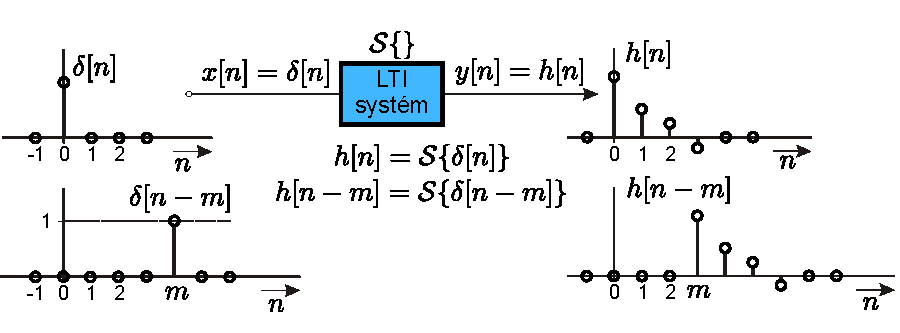
\includegraphics[scale=0.8]{impulzni_odezva.pdf}
         \caption[Impulzní odezva]{Odezva kauzálního diskrétního systému na jednotkový impulz
                  $\delta[n]$ a posunutý impulz $\delta[n-m]$}
        \label{SAS:fig_odezva3}
      \end{figure*}
  
      Postupná úprava rovnice (\ref{SAS:eq_odezva_skok2}) je umožněna díky linearitě systému,
      kterou budeme studovat pro obecný vstupní signál
      \begin{equation}\label{SAS:eq_odezva_na_diskretni_signal}
        x[n]=\sum_{m=-\infty}^\infty x[m]\delta[n-m].
      \end{equation}
      Poznamenejme, že formou (\ref{SAS:eq_odezva_na_diskretni_signal}) lze zapsat každý diskrétní
      signál.
     
      %---------------------------------------------
      \pgfplotsset{
    standard/.style={%Axis format configuration
        axis x line=middle,
        axis y line=middle,
        enlarge x limits=0.15,
        enlarge y limits=0.15,
        every axis x label/.style={at={(current axis.right of origin)},anchor=north west},
        every axis y label/.style={at={(current axis.above origin)},anchor=north east},
        every axis plot post/.style={mark options={fill=white}}
        }
  }
  \begin{figure}[hb!]
    \centering
    \subfloat[ ]   { %Unit step squence
      \begin{tikzpicture}
        \begin{axis}[%
          scale=0.45,
          standard,
          domain = 0:15,
          samples = 16,
          xlabel={\(n\)},
          ylabel={\(1[n]\)},
          ymin=0,
          ymax=1.1]
          \addplot+[ycomb,blue,thick] {1};
        \end{axis}
      \end{tikzpicture}
    }
    \subfloat[ ]   { %Sampled sine squence
      \begin{tikzpicture}
         \begin{axis}[%
            scale=0.45,
            standard,
            domain = 0:15,
            samples = 16,
            xlabel={$n$},
            ylabel={$x[n]$},
            ymax=1.1]
            \addplot+[ycomb,blue,thick] {sin(5*180*x/25)};
         \end{axis}
      \end{tikzpicture}
    }
    \caption[Posloupnost jednotkového a obecného signálu]{Posloupnost jednotkového skoku $1[n]$
             a signálu $x[n]$}
    \label{SAS:fig_odezva4}    
  \end{figure}

      % \label{SAS:fig_odezva4}
      %---------------------------------------------
      
      Na obr. \ref{SAS:fig_odezva4} znázorněna souvislost mezi posloupností jedniček a diskrétním
      sig\-ná\-lem. \emph{Posloupnost jedniček tvoří bázi pro diskrétní signály}. Každá komponenta
      diskrétního signálu je vyjádřena součinem $x[m]\delta[n-m]$. V uvedeném příkladě jde o
      posloupnost příslušnou jednotkovému skoku
      \begin{equation}\label{SAS:eq_odezva5}
        1[n]=\sum_{m=0}^{15}\delta[n-m]
      \end{equation}
      a odpovídající posloupnost konečného signálu
      \begin{equation}\label{SAS:eq_odezva6}
        x[n]=\sum_{m=0}^{15}x[m]\delta[n-m].
      \end{equation}
  
      Princip superpozice dovoluje získat odezvu systému jako sumu odezev na jednotlivé dílčí
      součásti vstupního signálu, které v rovnici (\ref{SAS:eq_odezva_na_diskretni_signal}) tvoří
      vážené jednotlivé impulzy, ze kterých je signál složen
      \begin{align}
        y[n]=\mathcal{S}\{x[n]\}
          &=\mathcal{S}\{\sum_{m=-\infty}^{\infty}x[m]\delta[n-m]\}  \nonumber \\
          &=\sum_{m=-\infty}^{\infty}x[m]\mathcal{S}\{\delta[n-m]\}. \label{SAS:eq_odezva7}
      \end{align}
      Protože platí (\ref{sas:eq_odezva3}) a v důsledku časové invariance vyplývá z rovnice
      \ref{SAS:eq_odezva7} \textbf{konvoluční suma} 
      \begin{equation}\label{SAS:eq_konvolucni_suma}
        y[n]=\sum_{m=-\infty}^{\infty}h[n-m]x[m]=\sum_{k=-\infty}^{\infty}h[k]x[n-k].
      \end{equation}
      Uvedli jsme, že u kauzálního systému závisí výstupní signál $y[n]$ pouze na současných a
      minulých hodnotách vstupního signálu $x[n], x[n-1], x[n-2], \cdots ,$ takže v konvoluční sumě
      \ref{SAS:eq_konvolucni_suma}
      \begin{align}
        y[n]&=\sum_{k=-\infty}^{\infty}h[k]x[n-k]                              \nonumber \\
            &=\sum_{k=-\infty}^{-1}h[k]x[n-k] + \sum_{k=0}^{\infty}h[k]x[n-k]  \label{tky:eq001}
      \end{align}
      musíme položit všechny členy impulzní odezvy $h[k]=0$ pro $k<0$. Konvoluční suma pro
      lineární, časově invariantní a kauzální systém má pak tvar
      \begin{equation}\label{SAS:eq_konvolucni_suma3}
        y[n]=\sum_{k=0}^{\infty}h[k]x[n-k].
      \end{equation}
      Jestliže navíc budeme uvažovat vstupní a výstupní signály, které jsou nulové pro $n<0$ a
      $x[n]\neq0, y[n]\neq0$ pouze pro $n\geq0$, potom platí
      \begin{equation}\label{SAS:eq_konvolucni_suma4}
        y[n]=\sum_{k=0}^{n}h[k]x[n-k]=\sum_{k=0}^{n}x[k]h[n-k].
      \end{equation}
  
      \begin{figure}[ht!]
        \centering
        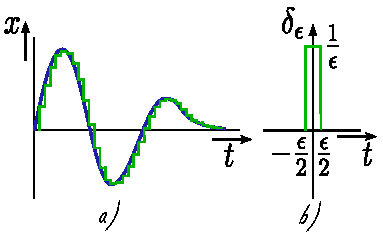
\includegraphics[width=0.7\linewidth]{bicak_aprox_spoj_sig_dirac.pdf}
        \caption[Aproximace spojitého průběhu signálu]{a) Aproximace spojitého průběhu signálu, b)
                 K odvození jednotkové impulsní funkce}
        \label{SAS:fig_Bicak_aprox_spoj_fce}
      \end{figure}
  
      Podobně můžeme postupovat i v analogovém případě a odvodit pro lineární časově invariantní 
      systém \emph{konvoluční integrál}. Vraťme se k výrazu \ref{SAS:eq_odezva_na_diskretni_signal} 
      kterým jsme vyjádřili libovolný diskrétní signál. Pro případ spojitého signálu vytvořme 
      analogickou formu zápisu využívající jednotkový impuls. Průběh obecného spojitého lze podle 
      obr. \ref{SAS:fig_Bicak_aprox_spoj_fce} aproximovat stupňovitým průběhem, který můžeme 
      vyjádřit jako sumu posunutých (zpožděných) impulsů. Výchozí aproximující impuls lze vyjádřit 
      vztahem
      \begin{equation}\label{SAS:eq_dirac}
          \delta_\epsilon(t)  =
            \begin{cases}
               \frac{1}{\epsilon} & \text{pro } |t| < \frac{\epsilon}{2},      \\
               0                  & \text{pro } |t| < \frac{\epsilon}{2} > 0
            \end{cases}
      \end{equation}
      a je znázorněn na obr. \ref{SAS:fig_Bicak_aprox_spoj_fce}. \emph{Jednotkový (Diracův) impuls} 
      má jednotkovou plochu. vat výrazem
      \begin{equation}\label{SAS:eq_dirac2}
        \delta_\epsilon(t) = \lim_{\epsilon\rightarrow0} \delta_\epsilon(t).
      \end{equation}
      Aproximaci spojitého průběhu $x(t)$ impulsy \ref{SAS:eq_dirac} lze vyjádřit rovnicí
      \begin{equation}\label{SAS:eq_spojit_aprox}
        x(t) = \sum_{m = -\infty}^\infty x(m\epsilon)\delta_\epsilon(t - m\epsilon)\epsilon .
      \end{equation}
      Zmenšování šířky impulsů $\epsilon \rightarrow 0$ se chyba aproximace zmenšuje a výraz přejde v limitu
      \begin{equation}\label{SAS:eq_spojit_aprox2}
        x(t) = \lim_{\epsilon\rightarrow0}
               \sum_{m = -\infty}^\infty x(m\epsilon)\delta_\epsilon(t - m\epsilon)\epsilon .        
      \end{equation}
      V limitě kdy $\epsilon\rightarrow0$, můžeme sumu nahradit integrálem, dále součin $m\epsilon$ 
      integrační proměnnou $\tau$ a $\epsilon$ jejím diferenciálem. Obdržíme
      \begin{equation}\label{SAS:eq_integral_aprox3}
        x(t) = \int_{-\infty}^{\infty}x(\tau)\delta(t-\tau)d\tau .
      \end{equation}
      Vztahem \ref{SAS:eq_integral_aprox3} jsme spojitý průběh signálu vyjádřili jako sumu 
      nekonečného počtu posunutých jednotkových impulsů váženou jeho okamžitými hodnotami. 
      Předpokládejme dále, že na vstup lineárního časově invariantního spojitého systému je 
      převeden jednotkový (Diracův) impuls a systém vytvoří odezvu $h(t)$. V případě obecného 
      vstupního spojitého signálu $x(t)$ aproximovaného vztahem \ref{SAS:eq_integral_aprox3}, bude 
      odezva analogového systému
      \begin{equation}\label{SAS:eq_integral_aprox4}
        y(t) = \int_{-\infty}^{\infty}x(\tau)h(t-\tau)d\tau 
             = \int_{-\infty}^{\infty}h(\tau)x(t-\tau)d\tau
      \end{equation}
      Uvedený integrál nazýváme \textbf{konvolucí} a velmi často ho označujeme jako 
      \begin{equation}\label{SAS:eq_konvoluce}
        y(t) = h(t)*x(t) .
      \end{equation}
      Funkce $h(t)$ představuje \emph{impulsní odezvu}. Jedná se o výstupní signál systému, na 
      jehož vstupu se uplatní Diracův impuls $x(t)=\delta(t)$. Platí totiž
      \begin{equation}\label{SAS:eq_h_plati}
        y(t) = \int_{-\infty}^{\infty}h(\tau)\delta(t-\tau)d\tau = h(t) . 
      \end{equation}     
      Z důvodů \emph{kauzality}, která vyjadřuje zachování příčinné posloupnosti událostí při 
      transformaci signálu ze vstupu na výstup, požadujeme
      \begin{align}\label{SAS:eq_kauzalita_pozadavky}
        h(t) &\neq  0 \text{   pro } |t| \geq0, \\
        h(t) &  =   0 \text{   pro } |t| < 0. 
      \end{align}    
      Potom můžeme konvoluční integrál \ref{SAS:eq_integral_aprox4} zapsat ve tvarem
      \begin{equation}\label{SAS:eq_konvolucni_integral}
         y(t) = \int_0^{\infty}h(\tau)x(t-\tau)d\tau .
      \end{equation} 
  
  \section{Popis spojitých a diskrétních systémů, pře\-no\-so\-vá funkce}
    \subsection{Spojité systémy}
      Lineární časově invariantní (LTI) spojitý systém je obecně popsán soustavou
      integrodiferenciálních rovnic s konstantními koeficienty, kterou lze postupným derivováním
      změnit na soustavu diferenciálních rovnic. Předpokládej\-me budící (ne\-zá\-vis\-lou) veličinu
      $x(t)$ a odezvou (závislou) výstupní veličinu $y(t)$, pak eliminací ostatních proměnných bude 
      soustava popsána jedinou diferenciální rovnicí s konstantními koeficienty tvaru
      \begin{equation}\label{SAS:eq_lin_dif_rov}
          \sum_{i=0}^na_i\frac{d^iy(t)}{dt^i}=\sum_{j=0}^mb_j\frac{d^jx(t)}{dt^j},
      \end{equation}
      kde $a_0, a_1, \cdots ,a_n$ a $b_0, b_1, \cdots ,b_m$ jsou konstanty charakterizující lineární
      systém. Obecné řešení $y(t)$ rovnice \ref{SAS:eq_lin_dif_rov} se sestává ze dvou částí, z 
      řešení \emph{homogenní rovnice} a \emph{partikulárního řešení}. K řešení je třeba znát 
      počáteční podmínky pro $y(t)$ a jeho derivace ve výchozím okamžiku.
  
      S použitím \emph{Laplaceovy transformace při nulových počátečních podmínkách} má rovnice
      (\ref{SAS:eq_lin_dif_rov}) tvar
      \begin{equation}\label{SAS:eq_L_tran_dif_rce}
        \sum_{i=0}^na_ip^iY(p)=\sum_{j=0}^mb_jp^jX(p),
      \end{equation}
      kde $X(p)=\mathcal{L}\{x(t)\}$ a $Y(p)=\mathcal{L}\{y(t)\}$ jsou Laplaceovy obrazy vstupní a
      výstupní veličiny, $p$ je Laplaceův operátor derivace a také komplexní kmitočet 
      $p=\sigma+j\omega$. Přenosová funkce $H(p)$ je definována jako podíl Laplaceova obrazu 
      výstupní veličiny $Y(p)$ ku obrazu vstupní veličiny $x(p)$, při nulových počátečních 
      podmínkách
      \begin{equation}\label{SAS:eq_Hp_popis}
          H(p)=\frac{Y(p)}{X(p)}.
      \end{equation}
      Vzhledem k rovnici (\ref{SAS:eq_L_tran_dif_rce}) je $H(p)$ racionálně lomenou funkcí tvaru
      \begin{align}
        H(p)&=\frac{b_mp^m+b_{m-1}p^{m-1}+\cdots+b_0}{a_np^n+b_{n-1}p^{n-1}+\cdots+a_0}  \nonumber\\
            &=\frac{\Pi_{j=1}^m(p-p_{0j})}{\Pi_{i=1}^n(p-p_{\infty i})}            \label{tky:eq002}
      \end{align}
      kde $p_{0j}$ jsou kořeny polynomu čitatele a představují \textbf{nulové body} a kořeny
      jmenovatele $p_{\infty i}$ jsou \textbf{póly} přenosové funkce, $H_0=\frac{b_m}{a_n}$ je
      násobná konstanta.
  
      Kmitočtové charakteristiky získáme z přenosové funkce substitucí
      \begin{equation}\label{SAS:eq_p_jomega}
          p = j\omega,
      \end{equation}
      ve které $\omega$ je úhlový kmitočet. Platí tedy
      \begin{align}
          H(p)\mid_{p = j\omega} 
            &=\frac{b_m(j\omega)^m+b_{m-1}(j\omega)^{m-1}                     
             +\cdots+b_0}{a_n(j\omega)^n+b_{n-1}(j\omega)^{n-1}+\cdots+a_0}      \nonumber \\
            &=M(\omega)e^{j\Phi(\omega)},                                        \label{tky:eq003}
      \end{align}
      kde $M(\omega)$ je \textbf{modulová charakteristika} a $\Phi(\omega)=\texttt{arg}H(j\omega)$ 
      se nazývá \textbf{fázová charakteristika}. Skupinové zpoždění je definováno jako záporně vzatá
      derivace fázové charakteristiky podle kmitočtu
      \begin{equation}\label{SAS:eq_skupinove_zpozdeni}
          \tau(\omega)=-\frac{d\Phi(\omega)}{d\omega}= - \frac{d \texttt{arg} H(j\omega)}{d\omega}.
      \end{equation}
      V předchozí kapitole jsme ukázali, že \emph{relace vstup/výstup LTI systému} souvisí
      pro\-střed\-nic\-tvím \emph{konvoluce}
      \begin{equation}\label{SAS:eq_popis_konvoluce}
          y(t)=\int_0^\infty h(\tau)x(t-\tau)d\tau = h(t)*x(t).
      \end{equation}
      Přenosová funkce je Laplaceova transformace impulzní odezvy $h(t)$
      \begin{equation}\label{SAS:eq_ht_Lap_trans_imp}
          H(p)=\mathcal{L}[h(t)]=\int_0^\infty h(t)e^{-pt}dt,
      \end{equation}
      pro kterou je splněn vztah
      \begin{equation}\label{SAS:eq_Yp}
          Y(p)=H(p)X(p).
      \end{equation}
      Přechodová odezva $s(t)$ je definována jako integrál impulzní odezvy
      \begin{equation}\label{SAS:eq_Prechod_odezva}
          s(t)=\int_0^th(\tau)d\tau,
      \end{equation}
      takže platí
      \begin{equation}\label{SAS:eq_st}
          s(t)=\mathcal{L}^{-1}\{\frac{H(p)}{p}\}.
      \end{equation}
      Algoritmus výpočtu impulzní odezvy z přenosové funkce je založen na výpočtu  reziduí a 
      rozkladu racionálně lomené funkce $H(p)=\frac{Q(p)}{N(p)}$ na částečné zlomky. Pokud má tato 
      funkce jednoduché póly, rozklad má tvar\footnote{Násobnost kořenů $N(p)$ neuvažujeme, protože 
      se v LTI obvodech neuplatňuje}.
      \begin{align}   %\label{tky:eq004}
         H(p)&=\frac{Q(p)}{N(p)} 
              =\sum_{\mu=1}^{n}\frac{k_\mu}{p-p_{\infty_\mu}}                  \nonumber \\
             &=\frac{k_1}{p-p_{\infty_1}}+\frac{k_2}{p-p_{\infty_2}}
               +\cdots+\frac{k_n}{p-p_{\infty_n}}                              \label{tky:eq004}
      \end{align}
      kde $k_\mu$ se nazývají rezidua v pólech $p_{\infty_\mu})$ a platí
      \begin{align}
        k_\mu &= \lim_{p\to p_{\infty_\mu}}(p-p_{\infty_\mu})\frac{Q(p)}{N(p)}  \nonumber \\
        \,    &= Q(p_{\infty_\mu})\lim_{p\to
                 p_{\infty_\mu}}\frac{1}{\frac{N(p)}{p-p_{\infty_\mu}}}=
                 Q(p_{\infty_\mu})\frac{1}{N'(p_{\infty_\mu})}                  \label{tky:eq006}
      \end{align}
      Impulzní odezva je pak dána vztahem
      \begin{equation}\label{sas:eq_impulzni_odezva}
        h(t)=\mathcal{L}^{-1}[H(p)]=\sum_{\mu=1}^nk_\mu e^{p_{\infty_\mu}t}
      \end{equation}
      Póly jsou obecně komplexní $p_{\infty_{\mu}}=\alpha_\mu+j\beta_\mu$, nebo reálné
      $p_{\infty_{\mu}}=\alpha_\mu$. Jsou to kořeny rovnice $N(p)=0$. Rovnice
      \ref{sas:eq_impulzni_odezva} je důležitá i proto, že z ní poznáme, zda analogová soustava je
      stabilní. Je patrné, že soustava bude stabilní, jestliže bude
      $\mathcal{R}\{p_{\infty_{\mu}}\}=\alpha_\mu<0$, tj. leží-li kořeny $p_{\infty_{\mu}}$ v
      otevřené levé polorovině komplexní roviny $p_{\infty_{\mu}}=\sigma+j\omega$. Imaginární osa
      $j\omega$ je mezí stability, pravá polorovina je oblastí nestability. Polynom, který má kořeny
      v levé otevřené polorovině se označuje \textbf{Hurwitzův polynom}.
      %---------------------------------------------------------------
      % !TeX spellcheck = cs_CZ Lineární obvody a systémy - Jan Bičák  - strana 10 Popis spojitých systémů
%===================================================================================================
\begin{mdframed}[style=mdexam]
  \begin{example}\label{tky:exam002}
    Lineární spojitý systém je dán zapojením dle obrázku. Určete:
    \begin{enumerate}[leftmargin=12pt,noitemsep]
      \item diferenciální rovnici pro odezvu $u_2(t)$, je-li na vstupu buzen napětím $u_1(t)$,
      \item přenos napětí $H(p)=\dfrac{U_2(p)}{U_1(p)}$,
      \item impulsní odezvu $h(t)$.
    \end{enumerate}

    {\centering
      \captionsetup{type=figure}
      \luafigure[1]{tky_fig008.pdf}
      \captionof{figure}{Zapojení obvodu RLC.}
      \label{tky:fig008}
    \par}
    \noindent\textbf{Řešení:} Pro zapojení dle obrázku \ref{tky:fig008} získáme metodou uzlových
    napětí integrodiferenciální rovnice pro uzly \texttt{A} a \texttt{B}:
    \begin{gather*}
      \begin{align*} %\label{tky:eq019}
        \shortintertext{uzel A:}
        \frac{u_3(t)-u_1(t)}{R}+\frac{1}{L}\int_0^t{[u_3(t)-u_2(t)]}\dd{\tau}+i_L(0_+) &= 0  \\
        \shortintertext{uzel B:}
        \frac{1}{L}\int_0^t[(u_2(t)-u_3(t))]\dd{\tau}+C\der{u_2}{t}-i_L(0_+)           &= 0
      \end{align*}
    \end{gather*}
    ve kterých \(i_L(0_+)\) je počáteční podmínka pro proud induktoru. Derivováním a eliminací
    $u_3(t)$ z původních rovnic dostaneme pro odezvu $u_2(t)$ diferenciální rovnici II. řádu.
    Začneme derivováním rovnice v uzlu \texttt{B} tj. \(\frac{d}{dt}(B)\):
    \begin{align*}
      u_2(t)-u_3(t)+LC\frac{d^2u_2(t)}{dt^2} &=0 \Rightarrow   \\
      u_2(t)+LC\frac{d^2u_2(t)}{dt^2}        &=u_3(t)
    \end{align*}
    Nyní můžeme z rovnice pro uzel \texttt{A} odstranit napětí \(u_3(t)\):
    \begin{align*}
      \frac{u_2(t)+LC\dfrac{d^2u_2(t)}{dt^2}-u_1(t)}{R}             &+    \\
      \frac{1}{L}\int_0^t{(LC\frac{d^2u_2(t)}{dt^2})}\dd{\tau}+i_L(0_+) &=  0 \\
      \shortintertext{}
      u_2(t)+LC\frac{d^2u_2(t)}{dt^2}-u_1(t)                        &+    \\
      RC\left[\frac{du_2(t)}{dt}\right]_0^t+Ri_L(0_+)               &=  0
    \end{align*}
    Při nulových počátečních podmínkách: $\left.\frac{du_2(t)}{dt}\right\rvert_{t=0}=0$,
    $i_L(0_+)=0$ dostaneme:
    \begin{equation*}
      \boxed{LC\frac{d^2u_2(t)}{dt^2}+RC\frac{du_2(t)}{dt}+u_2(t)=u_1(t)}
    \end{equation*}
    V Laplaceově transformaci platí:
    \begin{align*}
      \mathcal{L}\left[\frac{du_2(t)}{dt}\right]     &= pU_2(p)-u_2(0) \\
      \mathcal{L}\left[\frac{d^2u_2(t)}{dt^2}\right] &= p^2U_2(p)-pu_2(0)-\dot{u}_2(0),
    \end{align*}
    kde \(\dot{u}_2(0)=\left.\frac{du_2(t)}{dt}\right\rvert_{t=0}\). Při nulových počátečních
    podmínkách \(u_2(0) = 0\), \(\dot{u}_2(0) = 0\) a užitím Laplaceovy transformace přejde
    diferenciální rovnice na algebraickou rovnici:
    \begin{equation*}
      p^2LCU_2(p)+pRCU_2(p)+U_2(p)=U_1(p)
    \end{equation*}
    Odtud vyplývá \textbf{přenosová funkce} $H(p)=\frac{U_2(p)}{U_1(p)}$
    \begin{align}
      H(p) &=\dfrac{1}{p^2LC+pRC+1}                                   \nonumber \\
           &=\dfrac{1}{LC}\frac{1}{p^2+p\dfrac{R}{L}+\dfrac{1}{LC}}
            =\frac{Q(p)}{N(p)}                                        \label{tky:eq020}
    \end{align}
    K nalezení \textbf{impulsní odezvy} nejprve určíme póly přenosové funkce řešením rovnice
    $N(p)=0$
    \begin{align}
      p_{\infty_{12}} 
        &=\dfrac{\dfrac{R}{L}\pm\sqrt{\left(\dfrac{R}{L}\right)^2-\dfrac{4}{LC}}}{2}   \nonumber \\
        &=\frac{R}{2L}\pm\sqrt{\left(\frac{R}{2L}\right)^2-\frac{1}{LC}}          \label{tky:eq021}
    \end{align}
    a přenosovou funkci pak upravíme do tvaru
    \begin{equation*}
      H(p)=\frac{K}{(p-p_{\infty_1})\cdot(p-p_{\infty_2})}, \quad K=\frac{1}{LC}
    \end{equation*}
    kde \(K\) je násobná konstanta a \(p_{\infty_{1,2}}\) jsou její póly. 
    \begin{itemize}[leftmargin=12pt,noitemsep]
      \item Uvažujeme-li jednoduché póly a bude-li $R>2\sqrt{\frac{L}{C}}$ , potom z  rov.
            \ref{tky:eq021} vyplývají dva reálné různé póly. Přenosovou funkci tedy můžeme
            zapsat obecným tvarem:
            \begin{equation*}
              H(p)=\frac{K}{(p+a_1)\cdot(p+a_2)}=\frac{k_1}{p+a_1}+\frac{k_2}{p+a_2}
            \end{equation*}
            kde $p_{\infty_1}=-a_1,\, p_{\infty_2}=-a_2$, Rezidua  \(k_1\), \(k_2\) určíme z rov.
            \ref{tky:eq006}. 
            \begin{equation*}
              k_1=\frac{K}{a_2-a_1}, \quad k_2=\frac{K}{a_1-a_2}.
            \end{equation*}
            Impulsní odezvu pak vypočteme užitím rov. \ref{tky:eq023}.
            \begin{align*}
              h(t)&=\mathcal{L}^{-1}[H(p)]               \\
                  &=\frac{K}{a_2-a_1}e^{-a_1t}+\frac{K}{a_1-a_2}e^{-a_2t}
            \end{align*}
      \item Když bude $R<2\sqrt{\frac{L}{C}}$, obdržíme dvojici komplexně sdružených pólů a
            přenosovou funkci může obecně zapsat takto:
            \begin{equation*}
              H(p)=\frac{K}{(p+a_1)\cdot(p+a_2)}=\frac{k_1}{p+a-jb}+\frac{k_2}{p+a+jb}
            \end{equation*}
            kde $p_{\infty_1}=-a+jb$, $p_{\infty_2}=-a-jb$. Rezidua v pólech jsou dány výrazy
            $k_1=-\frac{jK}{2b}$, $k_2=\frac{jK}{2b}$. Impulzní odezvu opět určíme užitím rov.
            \ref{sas:eq_impulzni_odezva}.
            \begin{equation*}
              h(t) = \frac{Ke^{-at}}{2b}\left[j\cdot\left(-e^{jbt}+e^{-jbt}\right)\right]
            \end{equation*}
            \begin{gather*}
              \begin{align*}
                \,  &= \frac{Ke^{-at}}{2b}\left[j\cdot
                \left(\underline{-\cos(bt)}-j\sin(bt)+
                \underline{\cos(bt)}-j\sin(bt)\right)\right]                        \\
                \,  &= \frac{K}{b}e^{-at}\sin(bt)                                   
              \end{align*}
            \end{gather*}
    \end{itemize}
    
    Na obr. \ref{tky:fig009} je uvedena impulsní charakteristika uvaožovaného obvodu odpovídající
    hodnotám stavebních prvků: \(R=\SI{1}{\kohm}\), \(L=\SI{11.5}{\milli\henry}\),
    \(C=\SI{22.5}{\nano\farad}\). Výpis m-file \texttt{SAS\_exam\_02\_symb\_Hp\_solve.m} ukazuje
    symbolický způsob řešení operátorových obvodových rovnic pomocí \texttt{MATLABu}. Jde o filtr
    typu \textbf{dolní propust}, jehož přenosová funkce má tvar:
    $$H(p)= \frac{3.9506\cdot10^9}{p^2+8.8889\cdot10^4p+3.9506\cdot10^9}.$$
    %---------------------------------------------------------------
      \lstinputlisting[% style=luaMatlabStyle,
      caption={TKY\_exam\_02\_symb\_Hp\_solve.m}]{../src/TKY/matlab/SAS_exam_02_symb_Hp_solve.m}
    %---------------------------------------------------------------
    Impulzní charakteristiku obdržíme dosazením do vztahu \ref{tky:eq005}
    $$h(t)=\frac{K}{b}e^{-at}\sin(bt) =8.8890\cdot10^4e^{-4.4444\cdot10^4t}\sin(4.4444\cdot10^4t).$$
    
      {\centering
      \captionsetup{type=figure}
      \luafigure[1]{tky_fig009.pdf}
      \captionof{figure}{Impulzní charakteristika}
      \label{tky:fig009}
      \par}
    
    Z hlediska analýzy obvodů v kmitočtové oblasti je výhodné sestavovat obvodové rovnice (metodami
    uzlových napětí a smyčkových proudů) přímo v operátorovém tvaru. Kirchhoffovy zákony pro
    uzavřenou smyčku a proudu do uzlu pak mají tvar $$\sum_{k=1}^{n}U_k(p) = 0, \qquad
    \sum_{k=1}^{n}I_k(p) = 0.$$ Metodou uzlových napětí pro zapojení na obr. \ref{tky:fig008}
    obdržíme rovnice
    \begin{align}
      \frac{U_3(p)-U_1(p)}{R}+\frac{U_3(p)-U_2(p)}{pL} &=  0 \\
      pCU_2(p) + \frac{U_2(p)-U_3(p)}{pL}              &=  0 
    \end{align}
    Na rozdíl od \ref{tky:eq019} jde o algebraické rovnice, ze kterých eliminací uzlového napětí
    $U_3(p)$ vyplývá přenosová funkce \ref{tky:eq020} $$H(p) = \frac{U_2(p)}{U_1(p)} =
    \frac{1}{LC}\frac{1}{p^2+p\frac{R}{L} + \frac{1}{LC}}$$
    
    {\centering
      \captionsetup{type=figure}
      \luafigure[1]{tky_fig010.pdf}
      \captionof{figure}{Modulová, fázová charakteristika a skupinové zpoždění filtru}
      \label{tky:fig010}
      \par}    
    
    Dosazením za $p=j\omega$ lze z přenosové funkce vyjádřit modulovou charakteristiku $H(j\omega)$
    a fázovou charakteristiku $\Phi(\omega)= \texttt{arg} H(j\omega)$. Skupinové zpoždění vyplývá ze
    vztahu \ref{SAS:eq_skupinove_zpozdeni}. Modulová, fázová charakteristika a skupinové zpoždění
    jsou na obr. \ref{tky:fig010}.
    
    Filtr má maximálně plochou modulovou charakteristiku přenosu. Mezní kmitočet propustného pásma
    je $f_p = 10 kHz$, při kterém je $\abs{H(j\omega_p)}= 0.707$. Tato hodnota odpovídá poklesu
    modulové charakteristiky o $3 dB$.
    
    %---------------------------------------------------------------
    \lstinputlisting[% style=luaMatlabStyle,
      caption={TKY\_exam\_03\_Hp.m}]{../src/TKY/matlab/SAS_exam_03_Hp.m}
    %---------------------------------------------------------------  
  \end{example} 
\end{mdframed}
      %---------------------------------------------------------------

} %tikzset
%---------------------------------------------------------------------------------------------------
\printbibliography[title={Seznam literatury}, heading=subbibliography]
\addcontentsline{toc}{section}{Seznam literatury}